\documentclass{jsarticle}
\usepackage{color}
\usepackage{here}
\usepackage[dvipdfmx]{graphicx}
\title{Compare mesher}
\begin{document}


\maketitle 
\section*{Implicit surface meshing}
In order to obtain a deformed surface, we need to compute a triangle mesh implementation of the implicit surface computed with reconstruction algorithms.
\subsection*{Marching Cubes algorithm}

\subsection*{Delaunay based implicit surface meshing}

\section*{Experiment}
This experiment compared the running time of different meshing algorithms that applied mesh algorithm used sphere of 174 vertices, 344 faces. When sphere is input, we create sphere with different resolution using marching cube. This can create spheres with different number of vertices and different number of faces. As the marching cube grid size increases, the number of vertices increases, so we use it to create spheres with different vertices. The mesh algorithm with different number of vertices.  Our Delaunay is a Delaunay algorithm that based on CGAL. CGAL Delaunay meshes to the whole of the object. Our Delaunay is trying to speed up by detecting only the surface of the object and meshing it. The number of vertices and the number of faces in the marching cube of closed approximation hrbf may increase, but the execution time is not affected. The reason is that the spline is compact. There is no effect on execution time, because the function on the regular grid in the marching cube. CGAL Delaunay has increased the number of vertices and the number of faces. CGAL Delaunay is adding samples based on some condition\\
\\
\noindent
number of vertices: 480 \\
number of faces: 956 \\
Marching cube grid resolution: $16^3$\\
Closed-form approximation hrbf\\
\begin{table}[htb]
  \begin{tabular}{|l|c|c|c|} \hline
    Mesh algoritms & Marching cube & Our Delaunay & CGAL Delaunay \\  \hline
    Time[ms] & 40 & 30 & 4936\\ \hline
    Number of vertices and faces after mesh & 552, 1096 & 480, 954 &2102, 4196 \\ \hline
  \end{tabular}
\end{table}

\noindent
Poisson
\begin{table}[htb]
  \begin{tabular}{|l|c|c|c|} \hline
    Mesh algoritms & Marching cube & Our Delaunay & CGAL Delaunay \\  \hline
    Time[ms] & 7 & 25 & 1034\\ \hline
    Number of vertices and faces after mesh & 480, 956 & 480, 930 &1719, 3434 \\ \hline
  \end{tabular}
\end{table}

\noindent
number of vertices: 1992 \\
number of faces: 3980 \\
Marching cube grid resolution: $32^3$\\
Closed-form approximation hrbf\\
\begin{table}[htb]
  \begin{tabular}{|l|c|c|c|} \hline
    Mesh algoritms & Marching cube & Our Delaunay & CGAL Delaunay \\  \hline
    Time[ms] & 646 & 80 & 21669\\ \hline
    Number of vertices and faces after mesh & 2736, 5464 & 1992, 3970 &4769, 9530 \\ \hline
  \end{tabular}
\end{table}

\noindent 
Poisson
\begin{table}[htb]
  \begin{tabular}{|l|c|c|c|} \hline
    Mesh algoritms & Marching cube & Our Delaunay & CGAL Delaunay \\  \hline
    Time[ms] & 40 & 87 & 2118\\ \hline
    Number of vertices and faces after mesh & 2004, 4004 & 1992, 3628 &3887, 7766 \\ \hline
  \end{tabular}
\end{table}

\noindent
number of vertices: 8376 \\
number of faces: 16748 \\
Marching cube grid resolution: $64^3$\\
Closed-form approximation hrbf\\
\begin{table}[htb]
  \begin{tabular}{|l|c|c|c|} \hline
    Mesh algoritms & Marching cube & Our Delaunay & CGAL Delaunay \\  \hline
    Time[ms] & 24407 & 360 & 622310\\ \hline
    Number of vertices and faces after mesh & 13944, 27880 & 8376, 16754 &21143, 42274 \\ \hline
  \end{tabular}
\end{table}

\noindent
Poisson
\begin{table}[htb]
  \begin{tabular}{|l|c|c|c|} \hline
    Mesh algoritms & Marching cube & Our Delaunay & CGAL Delaunay \\  \hline
    Time[ms] & 221 & 256 & 16276\\ \hline
    Number of vertices and faces after mesh & 8378, 16752 & 8376, 14665 &20876, 41748 \\ \hline
  \end{tabular}
\end{table}

\noindent
number of vertices: 33696\\
number of faces: 67388 \\
Marching cube grid resolution: $128^3$\\
Poisson
\begin{table}[htb]
  \begin{tabular}{|l|c|c|c|} \hline
    Mesh algoritms & Marching cube & Our Delaunay & CGAL Delaunay \\  \hline
    Time[ms] & 1332 & 1133 & 73303\\ \hline
    Number of vertices and faces after mesh & 33696, 67388 & 33696, 55877 &76641, 153278 \\ \hline
  \end{tabular}
\end{table}

\noindent
number of vertices: 136224\\
number of faces: 272444\\
Marching cube grid resolution: $256^3$\\
Poisson
\begin{table}[htb]
  \begin{tabular}{|l|c|c|c|} \hline
    Mesh algoritms & Marching cube & Our Delaunay & CGAL Delaunay \\  \hline
    Time[ms] & 9763 & 3695 & 408205\\ \hline
    Number of vertices and faces after mesh & 136222, 272440& 136224, 185169 &343567, 686970 \\ \hline
  \end{tabular}
\end{table}

Graph showing time complexity for meshing algorithms. \\
The horizontal axis represents vertices and the vertical axis represents time in this graph.\\
Used reconstruction algorithm is Poisson.





\begin{figure}[h]
\begin{center}
\textbf{Marching cube, Our Delaunay and CGAL Delaunay time}
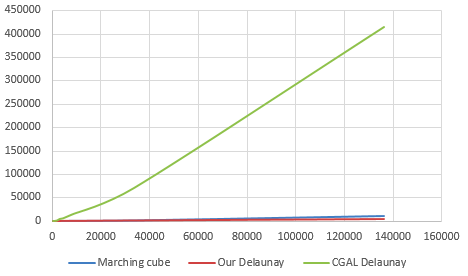
\includegraphics[width=10cm]{compare_mesher_graph.png}
\end{center}
Poisson surface reconstruction algorithm is O(log v) where v is the number of points in the input point-cloud. 
Marching cube time complexity is $O(n^3 log v)$. n is grid resolution. When the number of vertices is small, it is faster than other meshers. The more vertices the more it will take more time.\\
Our Delaunay's time complexity is $O(v^2 log v)$ . However, A paper of Attali and Boissonnat suggests that the time complexity in Delaunay triangulation is linear when points are sampled in 3D on the surface of the object. Thus, we should expect in practice a complexity of O(v log v). When the number of vertices is small, it is slower than the Marching cube, but as the number of points increases, it becomes the fastest meshing algorithm.\\
Time complexity is $O(V^3)$. CGAL Delaunay is adding samples based on some condition.  The increase in time when the number of vertices is increased is large, this was the slowest algorithm.
\section*{Conclusion}
Our Delaunay based implicit surface mesher is the fastest. If the number of vertices a few, it will not be a problem even with Marching Cube, but as the number of vertices increases, it is faster to use our Delaunay.
\end{figure}


\end{document}